\documentclass{article}
\usepackage{epsfig,graphicx,epsf,subfigure, amssymb, amsmath, float}
\usepackage{hyperref}
\usepackage[letterpaper, total={6.5in, 9in}]{geometry}
\author{Team Maintainabilityish: Oscar Wang, David Zhou, Andrew Gauthier, David Zhang}
\date{\today}
\title{ECE 458 Evolution 4 Write Up}
\begin{document}
\maketitle
\section{Design Choices}
\subsection{Ruby on Rails}
We had a lot to say about Ruby on Rails for the last three evolutions, but in retrospect, Ruby on Rails was probably one of the best possible choices for creating our application.  It was designed for creating web apps with ease, and all of our earlier complaints are mainly a result of our own lack of experience.  The philosophy behind Ruby on Rails is to save the developer as much time as possible and allow for quick changes and updates to their projects.  For the most part, this really showed during all of our evolutions.  Generating new models, controllers, or database migrations was as simple as typing a simple command into the shell script, and the gems we decided to incorporate did a lot of our work for us.  The use of embedded Ruby in our view files also allowed us to easily query information from the back end and generate HTML and Javascript using Ruby code.  None of us have taken a class on databases or have extensive experience with HTML, CSS, and Javascript, so the extra time we had to spend familiarizing ourselves with Ruby probably saved us a lot of time learning how to use these other technologies in the long run.  Because Ruby on Rails does so much for us--from setting up the MVC framework to allowing us to incorporate external packages by just adding a line to our Gemfile--some requirements could be finished in just a few lines of code.\par
Ruby is also a very readable language, or at least it should be when it is properly written.  We have done our best to make our code readable and intuitive to understand by keeping our methods short and modular and naming everything as clearly as possible.  However, we have definitely not taken full advantage of Ruby's capabilities; it is possible to write succint one-liners that make Ruby code read a lot like English.  We are also very inconsistent with our conventions.  Ruby has many synonyms: methods that do the exact same thing or perform very similar functions and different notation for code that accomplishes the same thing (many of these were introduced in new versions of Ruby as the language developed).  In general, we do not do things the ``Ruby way,'' and it is likely that a seasoned Ruby on Rails developer would be able to tell that we are relatively new to this by looking at our code.  Furthermore, a lot of the program logic in our controllers is probably very unconventional because there always seem to be easier ways of doing things that we have not discovered yet.  For example, in our most recent evolution, we discovered server side validations, which prevent the database from saving models when certain constraints are violated.  If we had known about this earlier, we probably would have used it for all of our error checking logic and cleaned up a lot of the ugly code in our controllers.  For our current evolution, validations are used to fix bugs in previous evolutions, but they also would have been perfect for preventing the creation of cycles in our heirarchies.  If we were to continue this project, one of the first things we would do is refactor our code to follow Ruby conventions and utilize these new techniques to clean up the code.\par
Of course, Ruby is also not without its downsides.  The lack of any typing makes the code less cluttered, but it is also quite frustrating when everything breaks because we are returning a variable of the wrong type.  The lack of an IDE is also both a boon and a blessing.  Having to use Sublime Text prevents us from coding with training wheels like we have been doing with Eclipse for the last few years and has forced us to think critically about the code we are writing.  Unfortunately, we also miss out of time-saving features like automatic line indentation and debugging tools.\par
Ultimately, we have a pretty good opinion of Ruby on Rails after working with it for a semester, and would definitely be interested in investing more time into learning how to use it properly.  It is a great framework for creating web applications as long as it is used properly.
\subsection{Twitter Bootstrap}
The decision we made to abandon React.js and implement the front end using only the Twitter Bootstrap was also one of the best decisions we have made.  We were already dealing with a learning curve from having to learn about Ruby on Rails, and adding Javascript and React on top of that was too much.  It led to our first evolution looking very, very primitive, and it probably would have still looked like that today if we continued down that path.  The Twitter Bootstrap was created by a company that built its website using Ruby on Rails, and incorporating Bootstrap front end elements into our framework was effortless.  
\section{Program Organization}
\subsection{MVC}
Overall, the default MVC setup that Ruby on Rails generates as soon as a new app is created has been great.  It is a time-tested approach for organizing programs for a reason.  Unfortunately, the code has definitely began to deviate a little from the ideal MVC setup in recent evolutions.  There is a lot of code in some of the view classes that should really go into the controllers, such as code that assigns values to variables or program control logic.  In addition, some of the methods in the controllers should really be integrated into the models.  This is one of the things we would refactor first if we were to continue working on this project.  In the future, we will do our best to create ``fat'' models to keep the controller code clean and readable, and prevent any program logic from ending up in the views.
\subsection{Models}
In order to get the hierarchy system to work, we added a node model that had a one to many relationship with resources. The node had a parent id, which was identical to the id of a specific resource, and the resources associated with each node were the children for that parent node. The one to many relationship worked out well because this meant each resource could only have at most one node, so only one parent, which prevented conflict. The only flaw with this approach was that we had to manually check for cycles, since a cycle would not make sense.  The front end displays all resources that do not have parents in the root of the folder system, so creating a cycle would remove the entire hierarchy from our folder system entirely.\par
We also added two new columns to our resource class for limited sharing.  Resources now also have a sharing level, which can be limited, unlimited, or exclusive, and a sharing level that indicates the maximum number of simultaneous reservations for limited resources.  It was surprisingly painless to implement this feature, as all updates to the models could be accomplished by generating migration files using rails scripts and only minimal modifications had to be performed in the controllers and views to create limited and unlimited resources.
\subsection{Views}
For this evolution, we added several new UI elements to give the user more information about what is happening.  For example, the resources of a reservation now tell the user how many simultaneous reservations are happening at that time for limited resources, and also tell the user which restricted resources are pending approval.  We also added a folder system to the front end, which allows for intuitive navigation of the application.  This required us to implement several new methods in our Reservations Controller, which we will describe in the next section.\par
Unfortunately, the view classes have also become quite messy after we have implemented all of this new functionality.  There is a lot of duplicated for for similar UI elements, such as the resources table that appears in both the Reservations and Resources pages.  We know how to fix this now using Ruby's render command, and if we could do things differently we would have just written the front end using modular components to begin with.  Furthermore, a lot of control logic is placed within the view classes when they belong in the controller.  We declared and manipulated a lot of variables in the front end just out of laziness, when we really should have moved as much of this kind of code into the controller for that view.  Ideally, all of the program logic should be placed within the controller except the loops that are required for getting data from the back end.
\subsection{Controllers}
We had to add a lot of new code to the controllers to get all of the new features to work.  However, as we stated earlier, a lot of this new code really belongs in our models.  For example, all of the code involving resource hierarchies, including the code that prevents cycles and causes all children to be reserved when the parent is reserved, are found in the Reservations Controller.  It would be better to simply put this code in the Reservation models and use the validations we mentioned earlier, because the create and update methods on our controller are getting very long.  We also created methods for navigating the folder system in the front end and placed this in the same helper class (SortHelper) used to manipulate Tags on the Resource and Reservation pages.  All of these methods perform operations on the parameters in the URL to render the appropriate resources on the page.  There is some complicated and unintuitive code in this class involving regular expressions, and perhaps the whole setup with parameters would benefit from some refactoring.
\section{Status}
This is definitely our best evolution to date.  It is the first time we can confidently say that we have implemented every single one of the new requirements, and we have also fixed all of the problems in previous evolutions to the best of our knowledge.  We have finally gotten OAuth2 authentication working and fixed the bug with overlapping reservations.\par
We have also done our best to fix any bugs that still remain, but there are almost certainly corner cases that we have missed.  All of the ones that we have discovered no longer cause any problems, but we definitely approached catching all of the bugs in the wrong way.  All of the glitches in our app are handled using additional logic in the controllers, but validations are really the best way to prevent our illegal states or violated assumptions.  Validations can be written to be called whenever a certain action is performed, much like the Observer/Observable design pattern.  They are also capable of preventing the action from occurring if some requirement is not met.  Using validations for everything would do wonders for preventing all of the weird corner cases we have found (such as tags persisting in the database after all resources of that tag have been deleted or the invisible groups associated with each user not properly being changed along with the user).  Unfortunately, we discovered this paradigm relatively close to the deadline for this evolution, and decided it was not worth rewriting all of our previous code and risking the possibility of creating new bugs, especially when everything was already working.  If we were to continue working on this project, this is definitely one of the first things we would like to change.
\section{Contributions}
\subsection{Evolution 4}
\subsection{Oscar Wang}
Worked on the frontend, backend for evolution 1 and set up the Heroku server. For evolution 2, worked on the backend. For evolution 3, set up the models for the expanding requirements. For evolution 4, worked on requirement 8.
\subsection{David Zhou}
I had the least experience coming into this, so I spent a lot of time learning about web development during the beginning of the semester and began contributing more and more as the semester progressed.  I wrote all of the write-ups and did most of the work on the front end.  For evolution 1, I tried to learn how to use React.js but ultimately abandoned it because it was difficult to integrate with Ruby on Rails.  This is why our front end was so primitive for the first evolution; I was also simultaneously trying to learn Ruby and Javascript and it may have been possible to use React if I had more time.  For evolution 2, I implemented a front end using the Twitter Bootstrap and was resposible for debugging and fixing issues.  For evolution 3, I continued to extend the front end to make everything more intuitive and transparent, and was also responsible for working on features we were previously unable to implement (such as the date-range selection and oauth2).  I also continued to be responsible for debugging.  For evolution 4, I implemented all of requirement 7 and the front end for requirement 8. I also continued to work on previously unimplemented features (i.e. anything we were penalized for in previous evolutions) and fixing bugs.
\subsection{Andrew Gauthier}
Completed the frontend and backend for evolution 1 and helped set up the Heroku server. For evolution 2, I worked on the implementing parts of the backend. In evolution 3, I helped design the models for the expanded requirements. During evolution 4, I helped with big picture design.
\subsection{David Zhang}
For Ev 1: Worked on designing and backend implementation. Ev 2: Primarily worked on planning and designing to account for new requirements. Ev 3: Extended the models and controllers to implement requirement 6 to reservations and management. Ev 4: Helped design and implement new models and and extend controllers for requirement 8
\section{Appendix}

\begin{figure}[h]
\centering
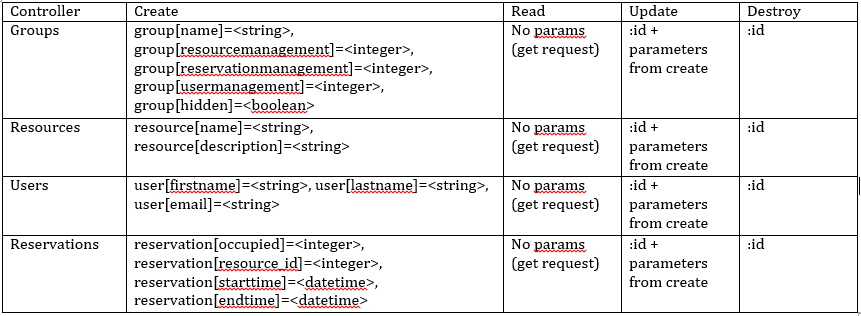
\includegraphics[width=6in]{table}
\caption{API}
\end{figure}

\end{document}

